
%*******************************************************************************
%*********************************** Conclusions ***************************
%*******************************************************************************
%!TEX root = 0.main.tex

\section{Conclusions}\label{sec:Chapter4}




\subsection{Experimental validation: SHREC17}
\label{sec:Chapter5:Experimental validation}
Gusset et al. \cite{Gusset} implemented the graph proposed in this work in a GCNN and three other rotation equivariant neural networks on a popular classification problem \cite{SHREC17}. The four models tested were the following: the original version of DeepSphere, Deepsphere \textit{Optimal} - obtained implementing the thresholding procedure described in this work in section \ref{sec:Chapter2:How to build a good graph} - and the traditional SCNNs of Cohen et al. \cite{SCNN} introduced in section \ref{sec:Chapter1:SCNN} and of Esteves et al. \cite{Esteves}
\paragraph{On the Equiangular sampling}. They compare with two different metrics  (accuracy, F1-score) the performances of these four rotation invariant models, while also comparing the speed of inference and of training of each model. Results are shown in table \ref{tab:SHREC17_class}.  It can be seen how \textit{DeepSphere Optimal} has \textit{always} the highest score between all the rotation equivariant models, no matter the evaluation metric. Furthermore, its performances in terms of speed of inference and training are second only to DeepSphere, remaining by far faster than the other two SCNNs. 
\begin{table}[ht]
	\centering
	\begin{tabular}{l|c c r r r}
		\multicolumn{1}{l}{} & \multicolumn{2}{c}{performance} & \multicolumn{1}{c}{size} & \multicolumn{2}{c}{speed}\\
		\cmidrule(lr){2-3} \cmidrule(lr){4-4} \cmidrule(lr){5-6}
		\multicolumn{1}{l}{Method} & Accuracy & F1-score & params & inference & training \\ \hline
		Cohen \emph{s2cnn\_simple} & 78.59 & 78.85 & 400k & 12ms & 32h\\
		Esteves \emph{sphericalcnn} & 79.18 & 79.36 & 500k & 9.8ms & 2h52\\ \hline
		Deepsphere & 73.36 & 73.67 & 190k & \textbf{0.98ms} & \textbf{43m} \\
		\textbf{Deepsphere \emph{Optimal}} & \textbf{80.42} & \textbf{80.65} & 190k & 1.0ms & 48m
	\end{tabular}
	\caption{Results form \cite{Gusset}. Performances of four rotation equivariant GCNNs and two SCNNs on the popular classification task SHREC17.}
	\label{tab:SHREC17_class}
\end{table}
\paragraph{On HEALPix }
Gusset et al. repeated the same test on the same dataset on a HEALPix sampling with $N_{side}=32$. Results can be seen in table \ref{table:results}.
\begin{table}[h!]
	\centering
	\begin{tabular}{ c|c|c } 
		& DeepSphere & DeepSphere \textit{Optimal} \\ 
		\hline
		accuracy & 82.23\% & 82.76\% \\ 
	\end{tabular}
	\caption{\label{table:results}Results form Gusset et al. Accuracy on the HEALPix sampling}
\end{table}
Being the new graph of DeepSphere Optimal more equivariant to rotations, we expected to see an improvement in the accuracy, as we did in the equiangular case. The fact that this improvement was not observed on HEALPix means that, in this case, the original DeepSphere graph $W$ \textit{is already sufficiently equivariant to rotations}. By this we mean that for this task, being equivariant to rotations of the low frequency eigenmodes is sufficient to obtain good results, and that being rotation equivariant to the higher frequencies does not lead to any improvement.

\subsection{Confront of different Discrete Laplacians on the equiangular sampling}
We conclude by showing how the different discrete Laplacians $\mathbf L$ illustrated so far compare in terms of equivariance error and computational time of the filter $\mathcal F(\mathbf f) = \mathbf L\mathbf f$. We can see how the four sparse discrete Laplacians are one order of magnitude faster than the two full Laplacians. The FEM Laplacian is able to reduce the equivariance error of the HKGL, and it manages to keep it low - around $0.5\%$ - even when using the sparse, lumped approximation $D^{-1}A$ while reducing the computational time of one order of magnitude. $D^{-1}A$ performs really well, and gets close to the performances of the graph Laplacian of Khasanova and Frossard. 
\begin{figure}[h!]
	\centering
	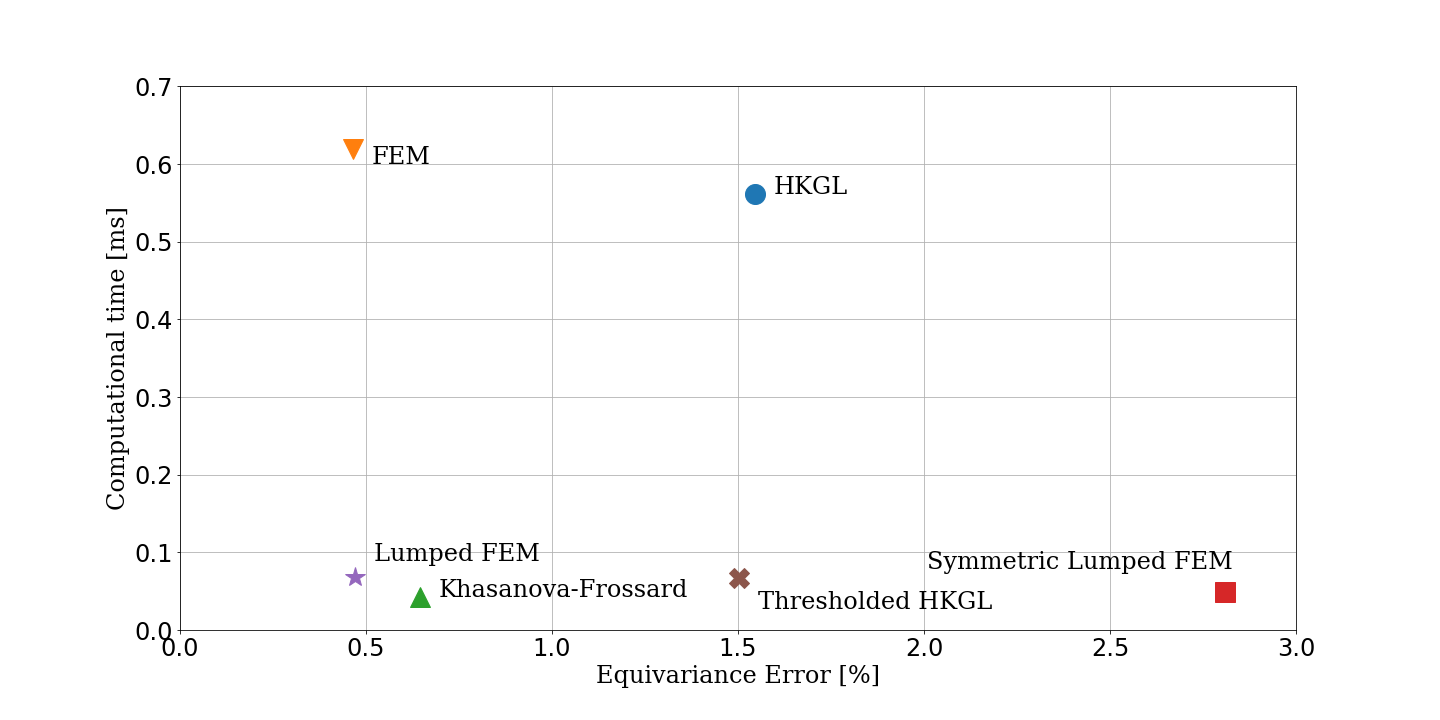
\includegraphics[width=\textwidth]{../codes/06.Equivariance_error/tradeoff.png}
	\caption{\label{fig:tradeoff}Trade-off between computational time and equivariance error for the filter $\mathbf L$ for different discrete Laplacians on the equiangular sampling}
\end{figure}

\subsection{Final considerations and future work}
In order not to confuse the notation between the FEM and the Graph approach we will be need a more precise notation than in the rest of this work. For this purpose, define a graph $G$, and its graph Laplacian by $L_G$. Define $V_G,\ \Lambda_G$ to be the solution of the eigenvalue problem
$$
L V_G = V_G \Lambda_G.
$$
Define the FEM stiffness matrix $A,\ (A)_{ij} = \int\nabla\phi_i\nabla\phi_j$ and the FEM mass matrix $B,\ (B)_{ij} = \int\phi_i\phi_j$. Define $V_{FEM}$ and $\Lambda_{FEM}$ to be the solution to the generalized eigenvalue problem 
$$
AV_{FEM} = BV_{FEM}\Lambda_{FEM}
$$
We saw that both in the graph and in the FEM filtering, filtering a sampled signal means approximating the Fourier transform $\hat{\mathbf f}$ through the multiplication of the signal $\mathbf f$ by the Fourier matrix - $V_G^T$ for the graph, $V_{FEM}^TB$ for the FEM - then applying a filter through a diagonal matrix $K$, and then applying the inverse Fourier transform - $V_G$ for the graph, $(V_{FEM}^TB)^{-1}$ for the FEM -. From these considerations follow that a polynomial filter $P_\kappa(\Lambda)$ is implemented in the graph domain by multiplying the signal $\mathbf f$ by a polynomial of the symmetric graph Laplacian $L_G$
$$
P_\kappa(L_G),
$$
and in the FEM domain (thanks to what explained in section \ref{sec:FEM filtering as a graph filtering}) by a polynomial of the matrix $B^{-1}A$
$$P_\kappa(B^{-1}A).
$$
The graph approach constrains the Fourier matrix $V_G$ to be orthogonal, while the FEM approach leaves to its Fourier matrix $V_{FEM}^TB$ more degrees of freedom. The fact that the mass matrix $B$ is constructed to \textit{exactly} represent the dot product in the Galerkin subspace $V_h$ and that the matrix $V_{FEM}$ converges to the sampled spherical harmonics makes it possible for the FEM to have a much better representation and interpretation of its discrete Fourier transform. How to interpret the fact that the graph approach constrains the Fourier matrix $V_G$ to be orthogonal is still not clear and subject of future work. However, even given these orthogonality constraints it is possible to design graphs with state-of-the-art performances, like the Khasanova-Frossard graph. Notice that this graph was obtained solving the optimization problem (\ref{eq:minimization frossard}) formulated directly in the spatial (vertex) domain, without relying on the spectral interpretation of the graph filtering, that in the case of a non uniform sampling presents the problems discussed above and it is still not clear.

